\documentclass{amsart}
\usepackage{graphicx, amsthm}
\usepackage{float}
\usepackage{enumerate}
\restylefloat{figure} 
\usepackage{tikz} 
\newcommand{\Z}{\mathbb{Z}}
\newcommand{\N}{\mathbb{N}}
\newcommand{\R}{\mathbb{R}}
\newcommand{\e}{\mathbf{e}}

\theoremstyle{definition} \newtheorem*{definition}{Definition} 
\theoremstyle{remark} \newtheorem*{ex}{Example} 


\title{Exercise set $3$, \\ MS-A0402, Foundations of Discrete Mathematics}
\begin{document}
\hspace{-1cm}
\maketitle
 
\section*{Explorative exercises}
I recommend to study the explorative problems before the first lecture of the week.

\subsection*{Problem 1} Let $B$ be an arbitrary set.
 \begin{enumerate}[a)]\item Let $f:\N\to B$ be an injective function. (Think of a few concrete examples.) Can you use $f$ to construct a surjective function $B\to \N$?
\item Let $g:\N\to B$ be a surjective function. (Think of a few concrete examples.) Can you use $g$ to construct an injective function $B\to \N$?
\item Can you do the same if $\N$ is replaced by an arbitrary set $A$? 
\end{enumerate}

 \subsection*{Problem 2}
The number of ways to select $k$ elements out of a set of size $n$ is denoted $\binom{n}{k}$
\begin{enumerate}[a)]
\item Argue that the number of ways to order a set of size $n$ is $$n!=n(n-1)(n-2)\cdots 2\cdot 1.$$
\item Argue that the number of ways to first select $k$ elements out of a set of size $n$, then order these elements, and then order the remaining $n-k$ elements, is $$\binom{n}{k}k!(n-k)!$$
\item Conclude that $$\binom{n}{k}=\frac{n!}{k!(n-k)!}.$$
\item What does this formula say when $k=0$, or when $k=n$? Do these formulas make sense?
\end{enumerate}

\subsection*{Problem 3}
Prove that the {\em binomial coefficients} $\binom{n}{k}$ satisfy the identity $$\binom{n}{k}=\binom{n-1}{k}+\binom{n-1}{k-1}.$$
\begin{enumerate}[a)]
\item Using the interpretation of $\binom{n}{k}$ as the number of combinations of $k$ out of $n$ elements.
\item Using the formula $\binom{n}{k}=\frac{n!}{k!(n-k)!}$
\end{enumerate}

 \subsection*{Problem 4}
What is the sum $\binom{n}{0}+\binom{n}{1}+\cdots + \binom{n}{n-1}+\binom{n}{n}$? If you do not see the answer immediately, first compute the sum for $n=3$, $n=4$, $n=5$, etc.. Can you explain this phenomenon combinatorially?

\pagebreak

 \section*{Homework}
The written solutions to the homework problems should be handed in on MyCourses by Monday 21.3 at 12:00. You are allowed and encouraged to discuss the exercises with your fellow students, but everyone should write down their own solutions.

\subsection*{Problem 1}
Let $P$ be the set of all Finland's presidents, and let $G$ be the set of all ordered pairs $(a, b) \in P \times P$ such that the president $b$ succeeded president $a$ in office.  Is $G$ the graph of a function?  Explain your answer.

\subsection*{Problem 2}
Find the domain and range of the function which assigns to each nonnegative integer its last digit.

\subsection*{Problem 3}
Eight people are to be seated around a table; the chairs don't matter, only who is next to whom, but right and left are different. Two people, X and Y, cannot be seated next to each other. How many seating arrangements are possible?

\subsection*{Problem 4}
Prove that for all $n \in \N$, $n \geq 9$, the following statement is true: for all $k \in \N$ with $0 \leq k \leq n$ we have
$$\binom{n}{k} < 2^{n-2}.$$
\textit{Hint:} You can use induction in $n$ with base case $n = 9$.


\vspace{0.2in}

\section*{Additional problems}

These do not need to be returned for marking.

\subsection*{Problem 1}
How many odd $5$-digit numbers (in the decimal system) have all their digits different?

\subsection*{Problem 2}
How many bit strings contain exactly eight 0s and ten 1s if every 0 must be immediately followed by a 1?

\subsection*{Problem 3}
Suppose that a department contains 10 men and 15 women. How many ways are there to form a committee with six members if it must have the same number of men and women?

\subsection*{Problem 4}
\begin{enumerate}[a)]
\item What is the coefficient of $x^2 y^3$ in the expansion of $(x+y)^{5}$?
\item What is the coefficient of $x^8 y^9$ in the expansion of $(x+y)^{17}$?
\item What is the coefficient of $x^8 y^9$ in the expansion of $(2x+3y)^{17}$?
\end{enumerate}

\subsection*{Problem 5}
\begin{enumerate}[a)]
\item How many relations on $\{1,2,\dots ,n\}$ are reflexive?
\item How many relations on $\{1,2,\dots ,n\}$ are symmetric?
\item How many relations on $\{1,2,\dots ,n\}$ are antisymmetric?
\end{enumerate}

\subsection*{Problem 6}
The {\em pigeonhole principle} is the following very simple but surprisingly useful observation: If a set with $n$ elements (``pigeons'') is partitioned into $m$ parts (``pigeonholes''), where $m<n$, then at least one of the pigeonholes contains at least two pigeons. Use this to show that, among 101 integers, there is a pair whose difference is divisible by 100.

\subsection*{Problem 7}
How many rectangles are bounded by the straight lines on a ``chessboard'' of size $n\times m$? (Example: On a board of size $1\times 2$, like below, there are 3 rectangles: the left one, the right one, and the entire board.)
\begin{center}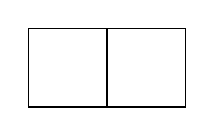
\begin{tikzpicture}
\draw [draw=black] (0,0) rectangle (2,1);
\draw (1,0) edge (1,1);
\end{tikzpicture}\end{center}

\subsection*{Problem 8}
Prove the identity $$\sum_{k=0}^n k\binom{n}{k}^2=n\binom{2n-1}{n-1}.$$ 

\subsection*{Problem 9}
Prove that there is no bijection $\N\to P(\N)$. Hint: Imitate the proof that there is no bijection $\N\to\R$.


\end{document}  